\section{Przypadek użycia}
\label{cha:usecase}

Zaprojektowany system będzie wykorzystywany w sposób pokazany na Rys. \ref{fig:usecase}. Celem implementacji jest stworzenie działającego przypadku użycia \quotedblbase Pobranie informacji o pacjencie\textquotedblright, który będzie wykorzystywany przez więcej niż jednego  \quotedblbase aktora (Doktor)\textquotedblright, a dane będą składowane w centralnej bazie.

\end{multicols}
\begin{figure}[h]
	\centering
	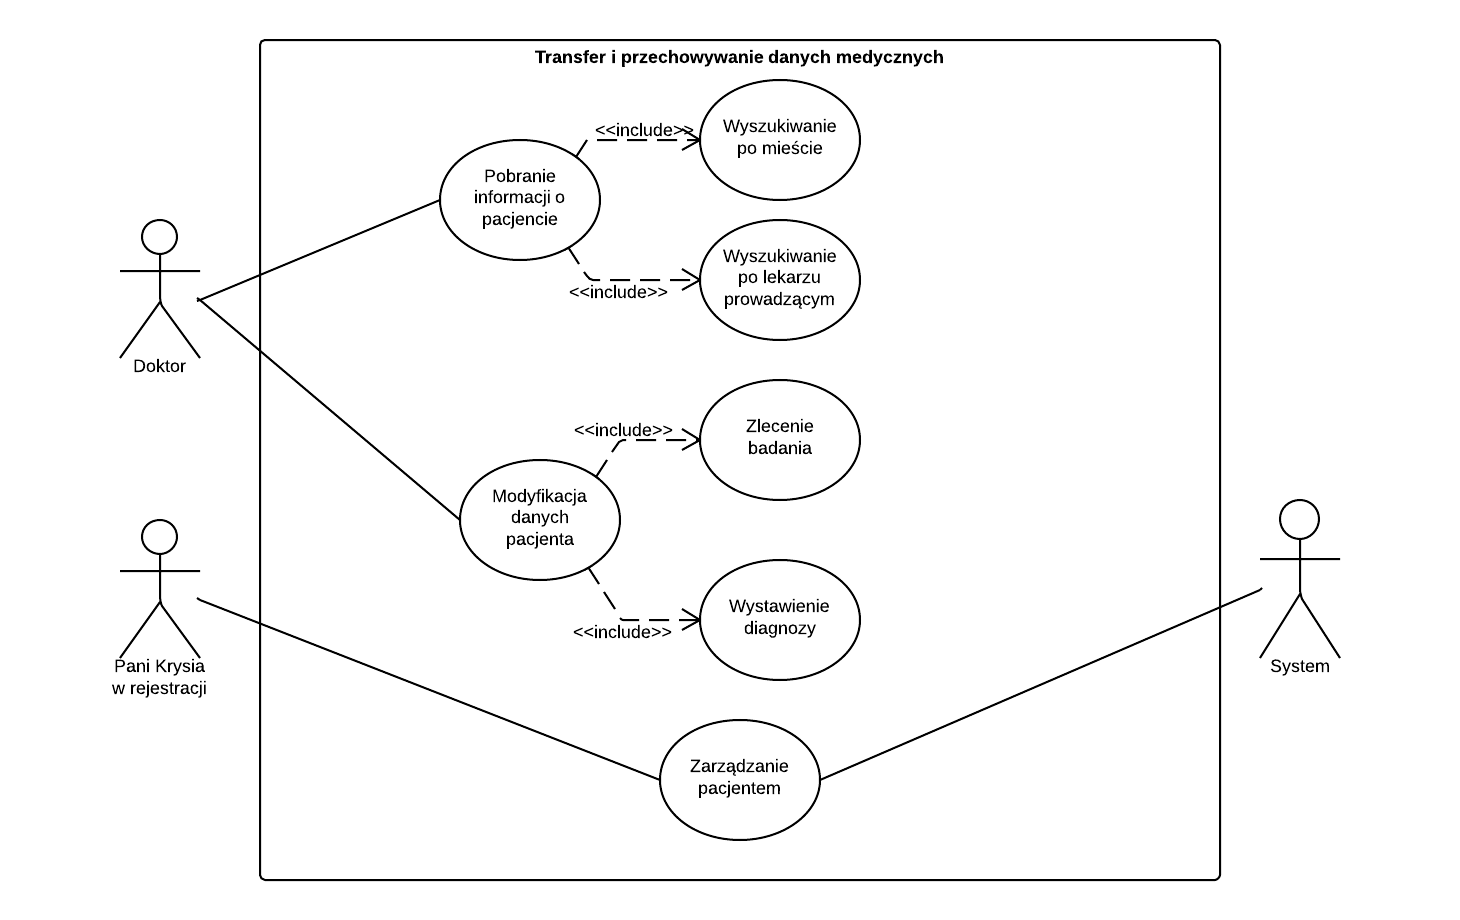
\includegraphics[width=\textwidth]{pics/UseCase}
	\caption{Diagram przypadków użycia}
	\label{fig:usecase}
\end{figure}
\begin{multicols}{2}

\subsection{Pobranie informacji o pacjencie}
\label{cha:patientinfo-usecase}

\subsubsection{Opis}
Przypadek użycia \quotedblbase Pobranie informacji o pacjencie\textquotedblright (Rys. \ref{fig:usecase}) przedstawia jedną z możliwych interakcji klienta (w tym wypadku lekarza) z systemem. Klient ma możliwość przefiltrowania pacjentów wg. miast i lekarzy prowadzących (lekarz może mieć pacjentów w róznych miastach).

\subsubsection{Zapytania SPARQL}
Przykładowe zapytanie użyte do pobrania pacjentów z danego miasta:
\begin{lstlisting}
SELECT ?patient WHERE { ?patient hl7:livesIn hl7:Nazwa_miasta }
\end{lstlisting}

\subsubsection{Implementacja po strone klienta - JAVA}